\documentclass[11pt,a4paper]{article}

\usepackage[headsep=1cm,headheight=3cm,left=3.5cm,right=3.5cm,top=2.5cm,bottom=2.5cm,a4paper]{geometry}

\linespread{1.3}
\setlength{\parindent}{0pt}
\setlength{\parskip}{1em}

\usepackage[spanish]{babel}
\usepackage[utf8]{inputenc}

%% Fuentes personalizadas para utilizar con XeTeX
\usepackage[sfdefault]{roboto}
\usepackage[scaled=0.9]{DejaVuSansMono}
\usepackage[T1]{fontenc}

\usepackage{enumitem}
\setlist[itemize]{leftmargin=*}
\setlist[enumerate]{leftmargin=*}

\usepackage{changepage}

\newcommand{\term}[2]{\textbf{#1}\quad#2}

\newcounter{ActCounter}
\newcommand{\act}[1]{\addtocounter{ActCounter}{1}\textbf{\sffamily ACT-\theActCounter}\quad#1\\}

\newcounter{CUCounter}
\newcommand{\cu}[1]{\addtocounter{CUCounter}{1}\textbf{\sffamily CU-\theCUCounter}\quad#1\\}

\usepackage{tabularx}
\usepackage{float}
\usepackage{adjustbox}

\newenvironment{itemizenomargins}
    {\begin{minipage}[t]{1\linewidth}\begin{itemize}}
    {\end{itemize}\end{minipage}}

\title{Práctica 4: Diseño \large\\ Fundamentos de Ingeniería del Software}
\author{Sofía Almedia Bruno \and José Antonio Álvarez Ocete \and Miguel Lentisco Ballesteros \and Simón López Vico \and José María Martín Luque}

\begin{document}

\maketitle

\section{Diagrama de clases}

Adjuntamos la figura del diagrama de clases a parte para una mejor visualización de la misma. \\

\begin{figure}[H]
	\centering
	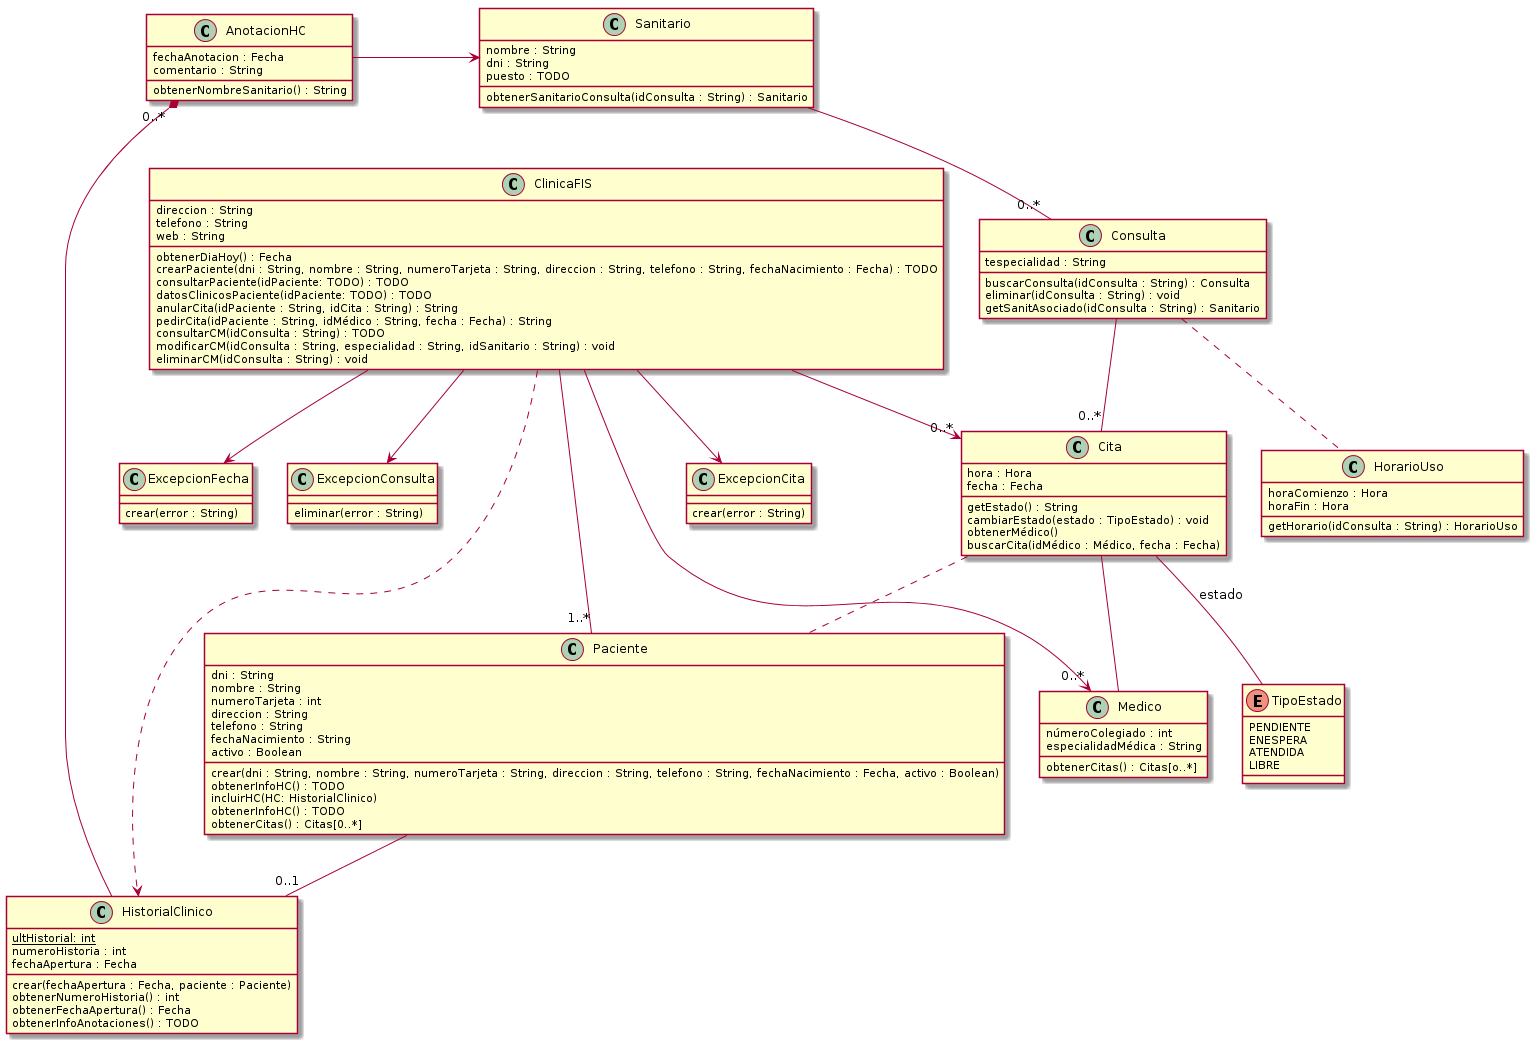
\includegraphics[width=\textwidth,height=\textheight,keepaspectratio]{Diagramas/diagramaClases}
\end{figure}

\section{Diagramas de Sofía Almeida}

\begin{figure}[H]
	\caption{anularCita}
	\centering
	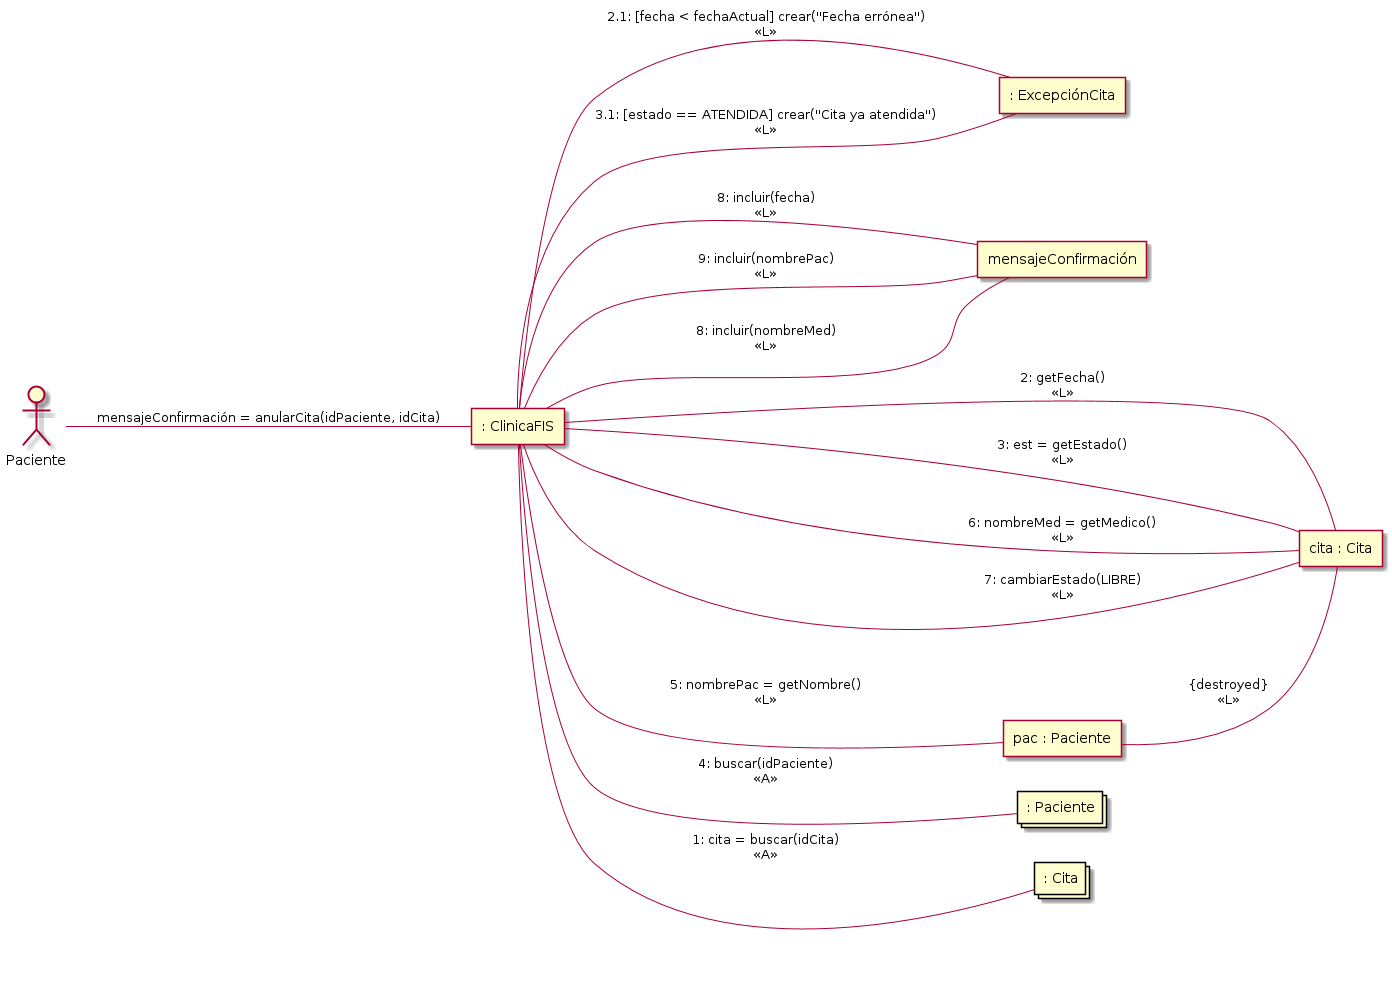
\includegraphics[width=\textwidth,height=\textheight,keepaspectratio]{Diagramas/anularcita}
\end{figure}

\begin{figure}[H]
	\caption{pedirCita}
	\centering
	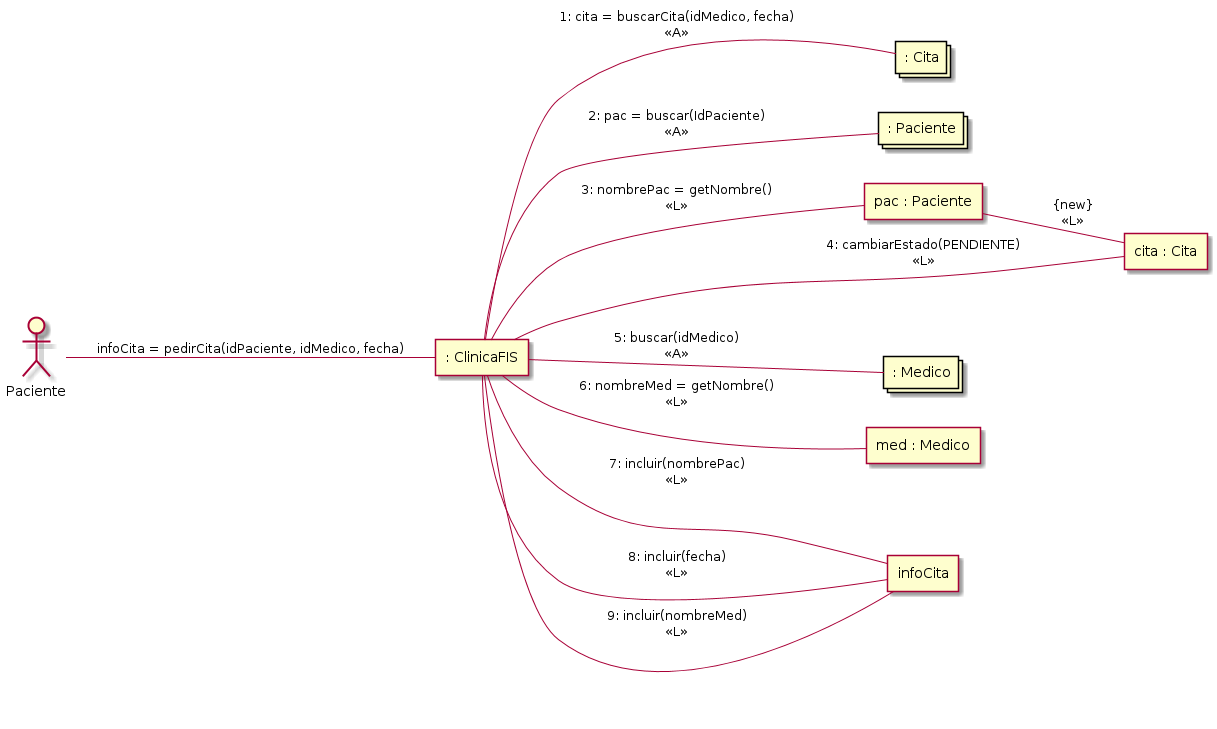
\includegraphics[width=\textwidth,height=\textheight,keepaspectratio]{Diagramas/pedircita}
\end{figure}

\begin{figure}[H]
	\caption{obtenerPosiblesCitas}
	\centering
	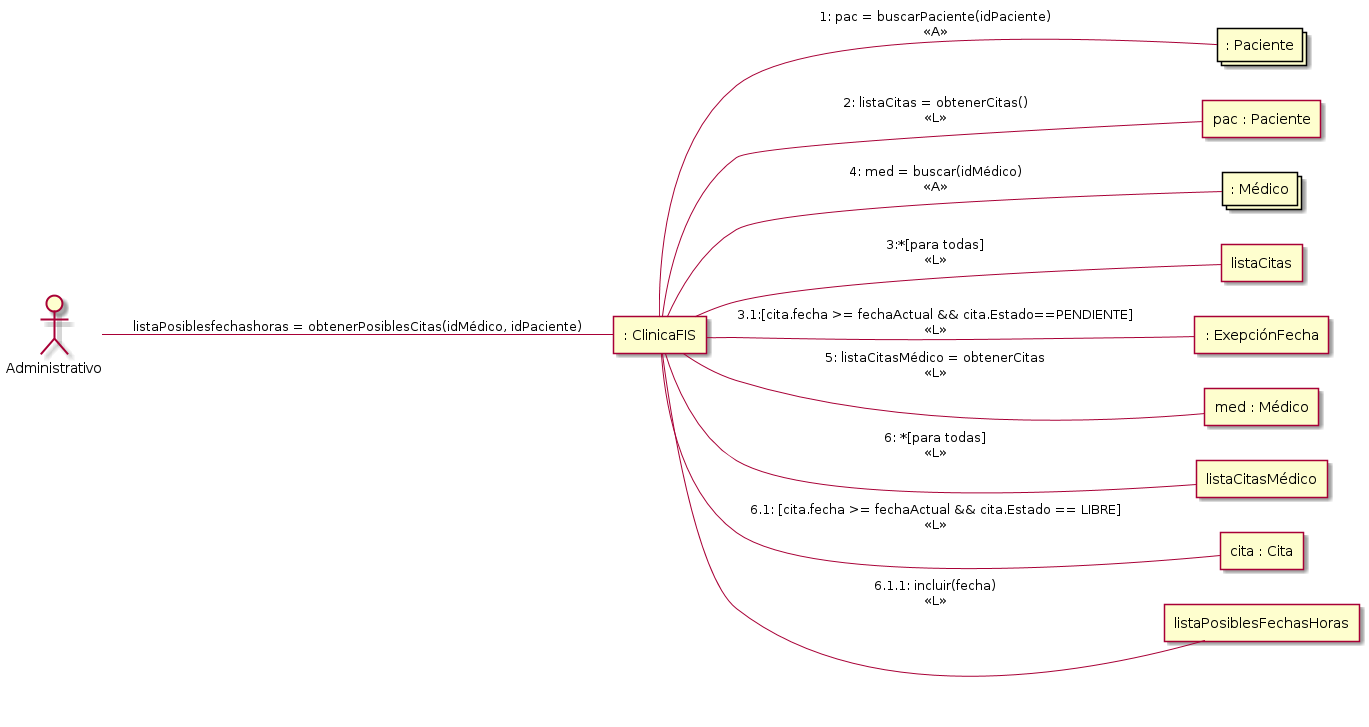
\includegraphics[width=\textwidth,height=\textheight,keepaspectratio]{Diagramas/obtenerposiblescitas}
\end{figure}

\section{Diagramas de José Antonio Álvarez}

\begin{figure}[H]
	\caption{modificarPaciente}
	\centering
	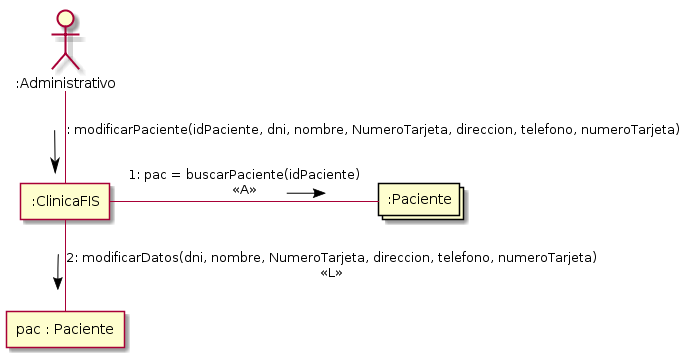
\includegraphics[width=\textwidth,height=\textheight,keepaspectratio]{Diagramas/modificarPaciente}
\end{figure}

\begin{figure}[H]
	\caption{consultarCitas}
	\centering
	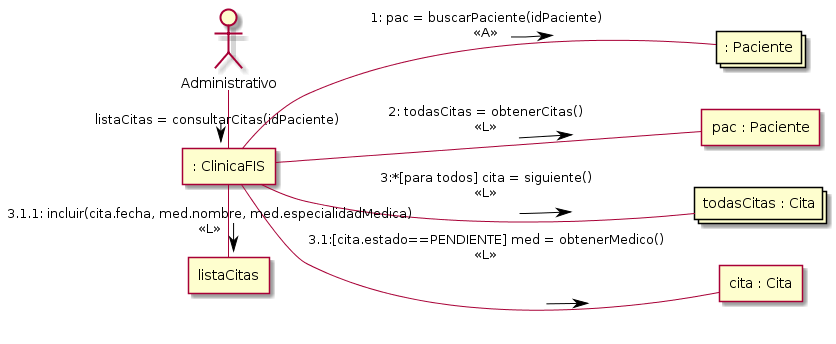
\includegraphics[width=\textwidth,height=\textheight,keepaspectratio]{Diagramas/consultarCitas}
\end{figure}

\begin{figure}[H]
	\caption{eliminarPaciente}
	\centering
	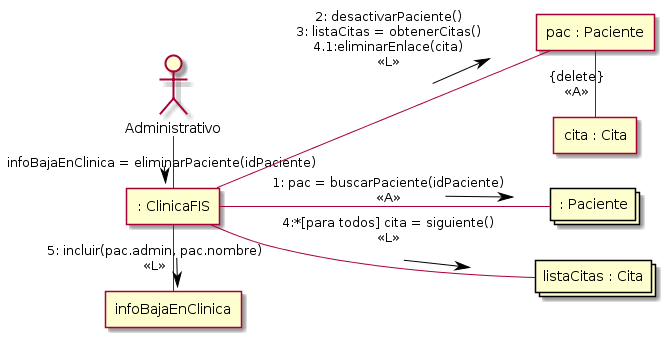
\includegraphics[width=\textwidth,height=\textheight,keepaspectratio]{Diagramas/eliminarPaciente}
\end{figure}

\section{Diagramas de Simón López Vico}

\begin{figure}[H]
	\caption{consultarCM}
	\centering
	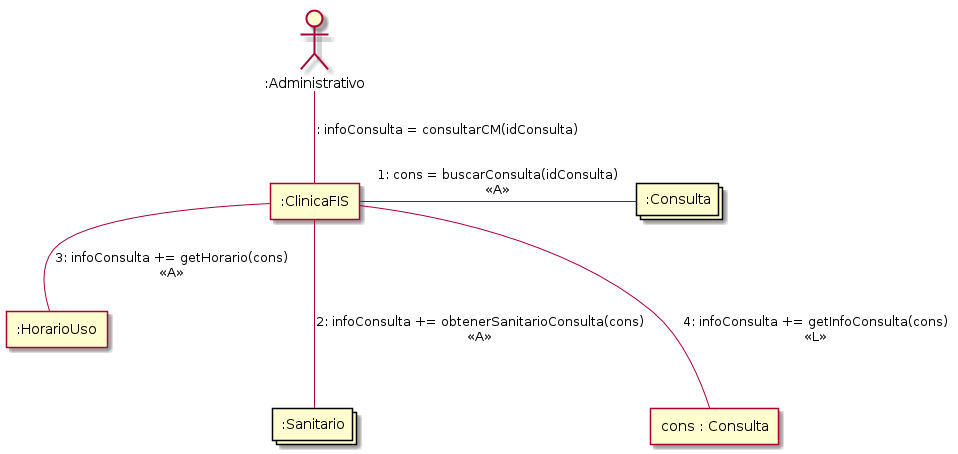
\includegraphics[width=\textwidth,height=\textheight,keepaspectratio]{Diagramas/consultarCM}
\end{figure}

\begin{figure}[H]
	\caption{modificarHorarioCM}
	\centering
	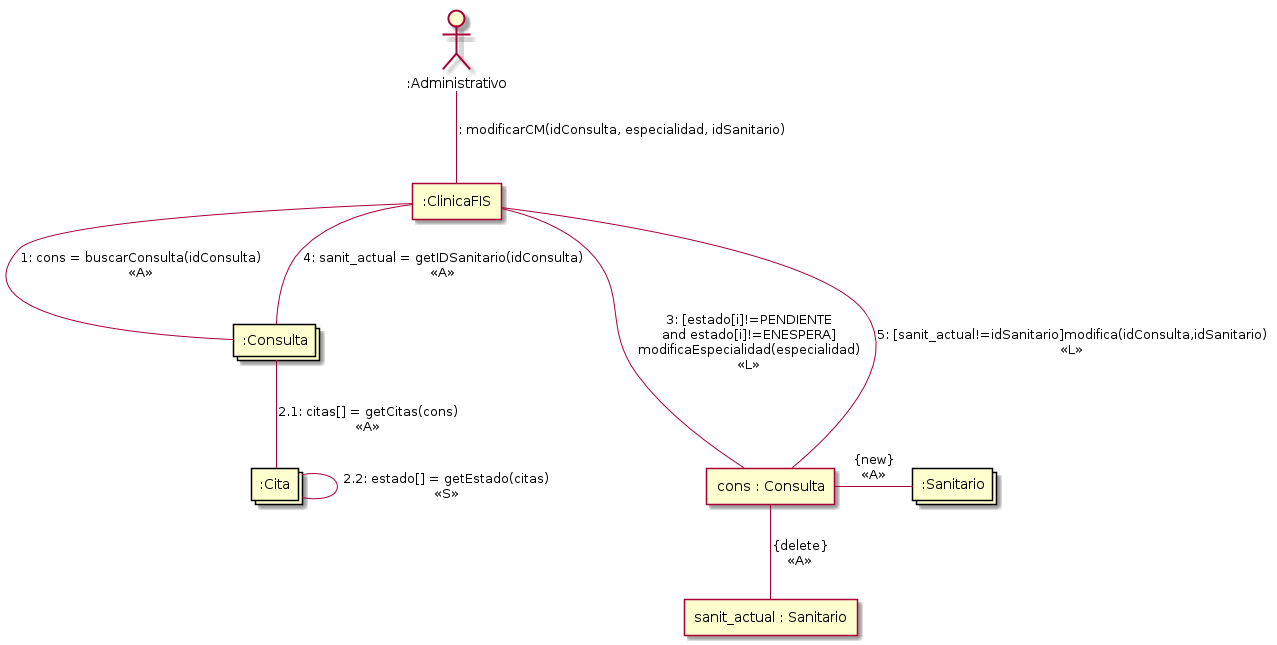
\includegraphics[width=\textwidth,height=\textheight,keepaspectratio]{Diagramas/modificarHorarioCM}
\end{figure}


\begin{figure}[H]
	\caption{eliminarCM}
	\centering
	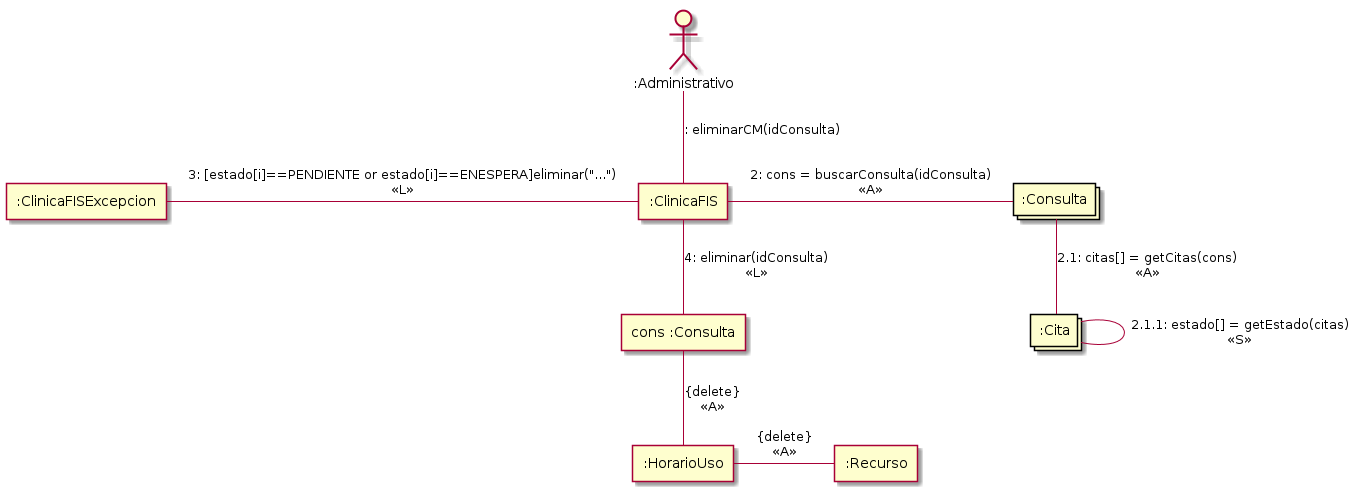
\includegraphics[width=\textwidth,height=\textheight,keepaspectratio]{Diagramas/eliminarCM}
\end{figure}


\section{Diagramas de José María Martín}

\begin{figure}[H]
	\caption{diagnosticar}
	\centering
	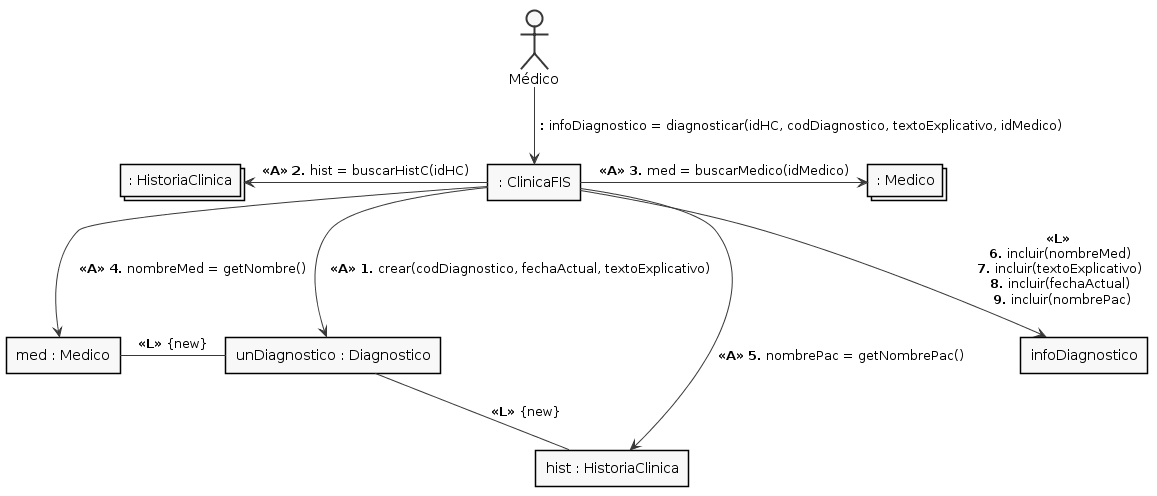
\includegraphics[width=\textwidth,height=\textheight,keepaspectratio]{Diagramas/diagnosticar}
\end{figure}

\begin{figure}[H]
	\caption{llamarSiguientePaciente}
	\centering
	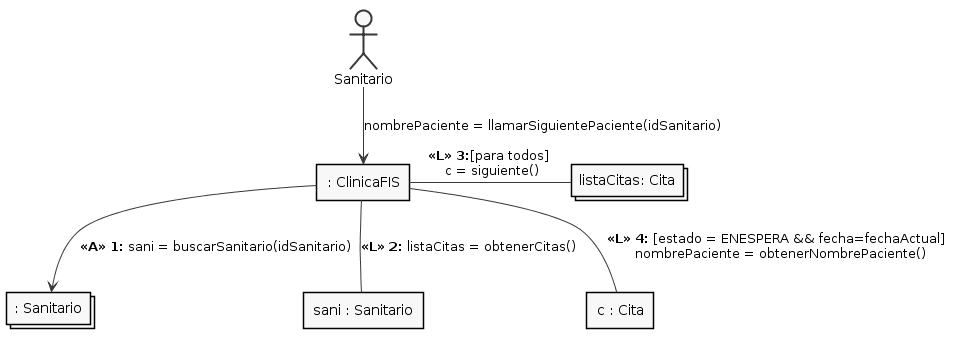
\includegraphics[width=\textwidth,height=\textheight,keepaspectratio]{Diagramas/llamarsiguientepaciente}
\end{figure}

\begin{figure}[H]
	\caption{terminarConsulta}
	\centering
	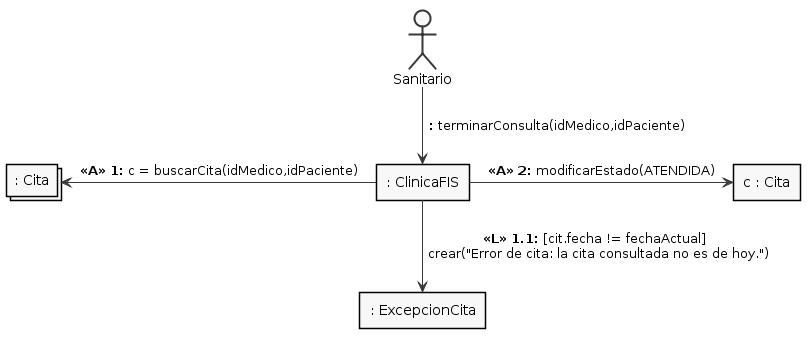
\includegraphics[width=\textwidth,height=\textheight,keepaspectratio]{Diagramas/terminarconsulta}
\end{figure}

\section{Diagramas de Miguel Lentísco}

\begin{figure}[H]
	\caption{consultarPaciente}
	\centering
	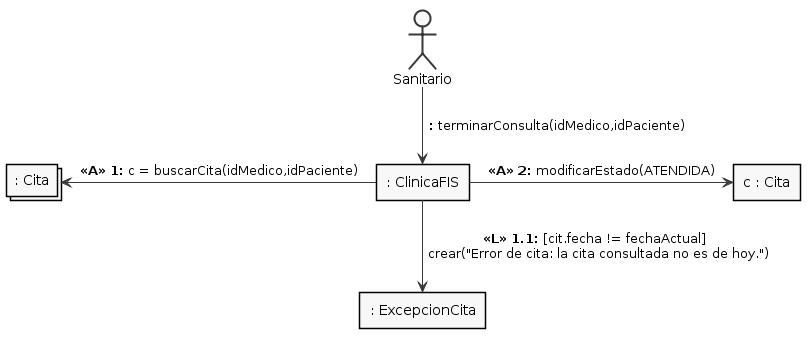
\includegraphics[width=\textwidth,height=\textheight,keepaspectratio]{Diagramas/terminarconsulta}
	%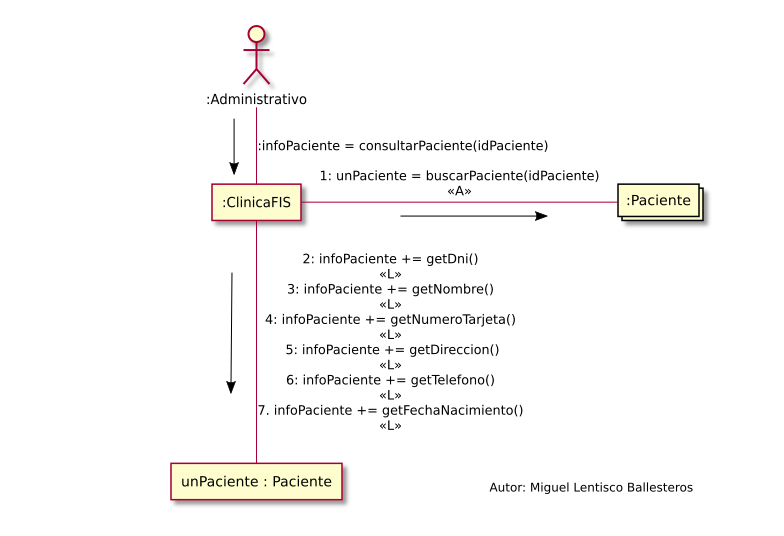
\includegraphics[width=\textwidth,height=\textheight,keepaspectratio]{Diagramas/consultarPaciente}
\end{figure}

\begin{figure}[H]
	\caption{crearPaciente}
	\centering
	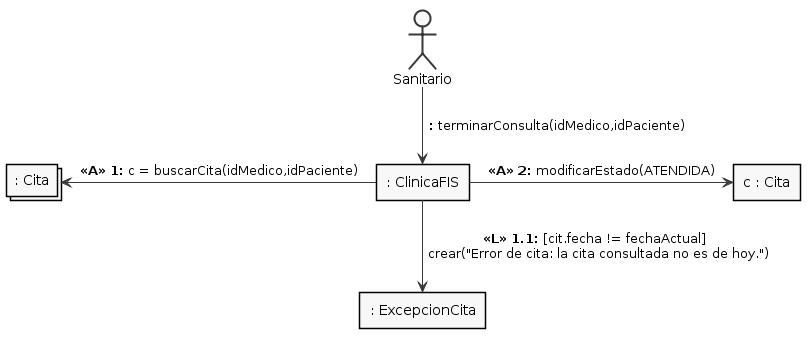
\includegraphics[width=\textwidth,height=\textheight,keepaspectratio]{Diagramas/terminarconsulta}
	%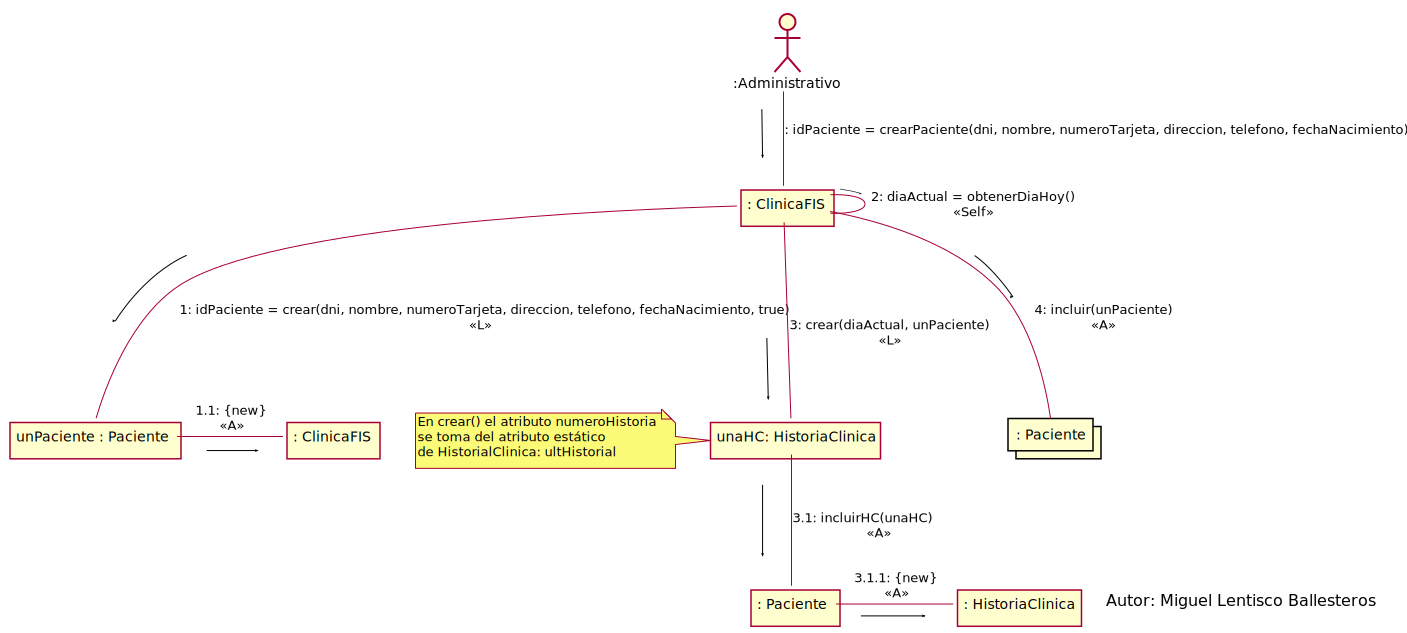
\includegraphics[width=\textwidth,height=\textheight,keepaspectratio]{Diagramas/crearPaciente.svg}
\end{figure}

\begin{figure}[H]
	\caption{datosClinicosPaciente}
	\centering
	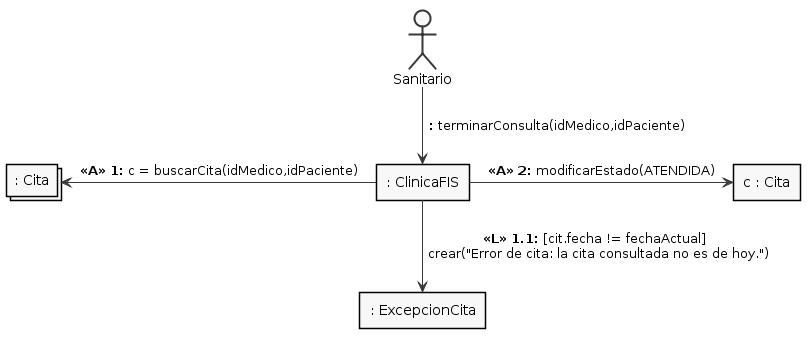
\includegraphics[width=\textwidth,height=\textheight,keepaspectratio]{Diagramas/terminarconsulta}
	%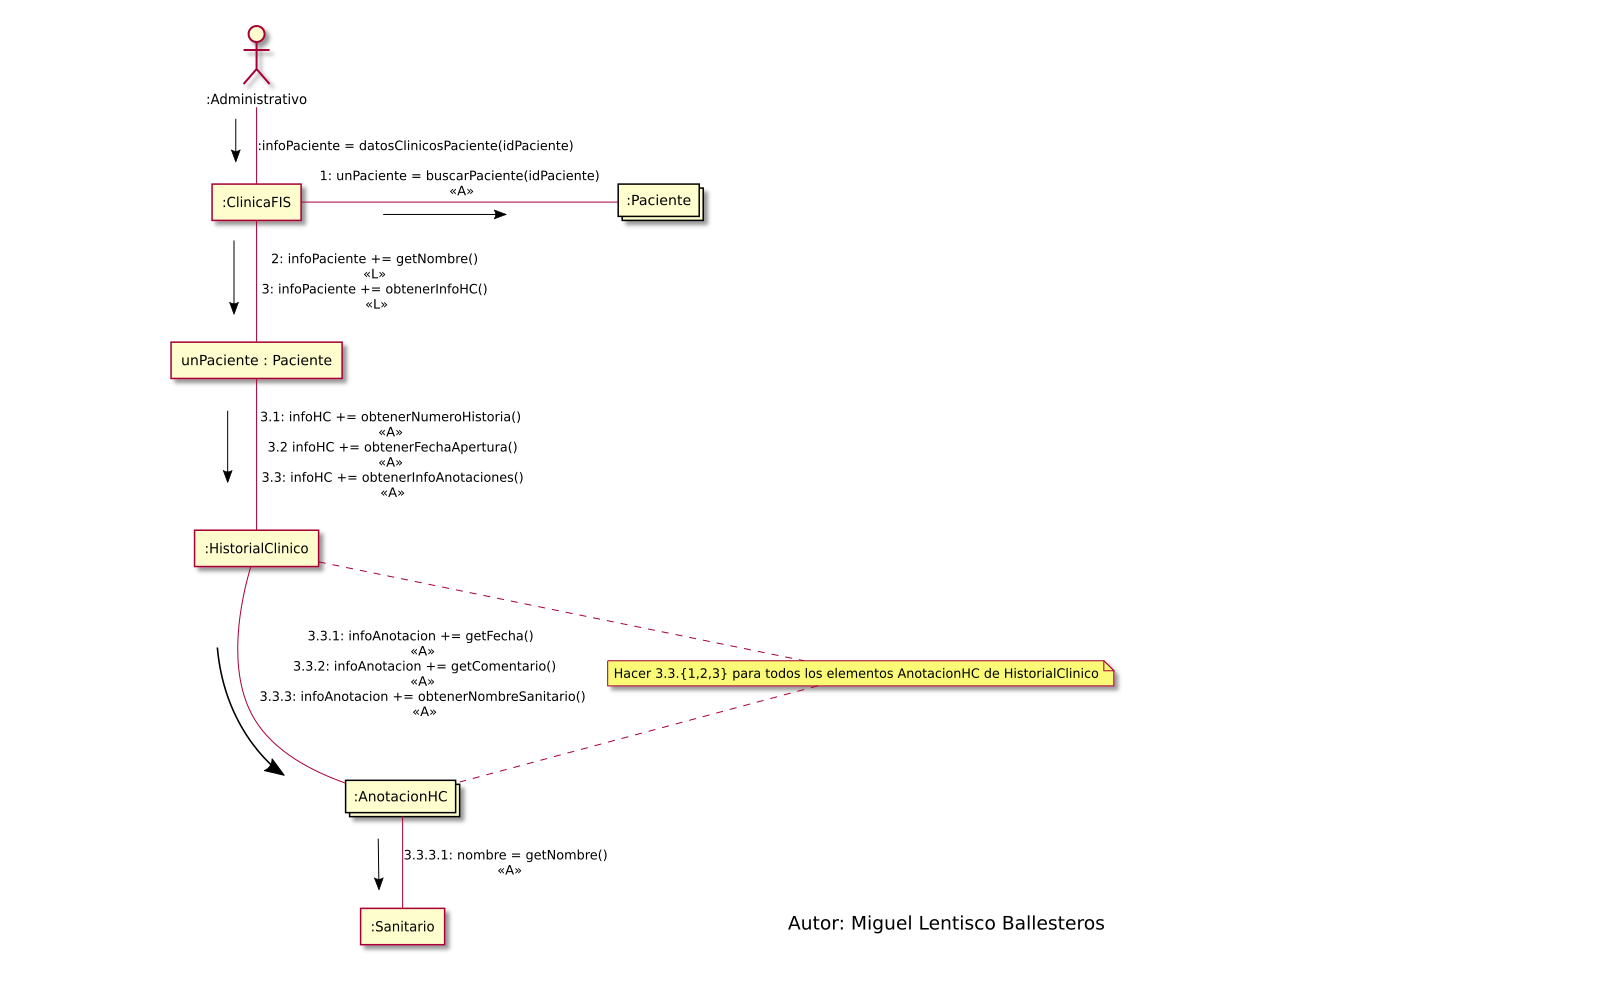
\includegraphics[width=\textwidth,height=\textheight,keepaspectratio]{Diagramas/datosClinicosPaciente}
\end{figure}

\end{document}
